\documentclass[11pt]{article}
\usepackage[a4paper,margin=1in]{geometry}
\usepackage[T1]{fontenc}
\usepackage{lmodern}
\usepackage{microtype}
\usepackage{amsmath,amssymb,amsthm}
\usepackage{booktabs,array,longtable}
\usepackage{enumitem}
\usepackage{xcolor,listings}
\usepackage{tikz}
\usetikzlibrary{positioning,arrows.meta}
\usepackage[hyphens]{url}
\usepackage[hidelinks]{hyperref}
\usepackage{cleveref}

\definecolor{codegray}{gray}{0.96}
\lstset{basicstyle=\ttfamily\small,backgroundcolor=\color{codegray},
  frame=single,framerule=0.2pt,columns=fullflexible,keepspaces=true,
  breaklines=true,showstringspaces=false,tabsize=4,
  aboveskip=0.8em,belowskip=0.8em}
\newcommand{\jsolv}{\textsc{JSOLV}}
\newcommand{\labels}{\mathcal{L}}
\newcommand{\powerset}{\mathcal{P}}
\newtheorem{proposition}{Proposition}

\title{JSOLV: Java Static Object Labelling\\for Verification\\
Application-Owned Value-State Contracts for Java}
\author{Jayanta Majumder \and Sambuddha Majumder}
\date{10 October 2026}

\begin{document}
\maketitle

\begin{abstract}
An ordinary Java type often says little about whether a value has passed through
the workflow stages required by its consumer. A document may have been persisted,
validated, and authenticated while remaining an ordinary document throughout.
JSOLV, ``Java Static Object Labelling for Verification'', implements a lightweight layer
for expressing and checking such facts. Application programmers declare their
label vocabulary in a two-key configuration file. A Maven plugin generates the
annotation classes before compilation; a generic annotation processor recognises
their shared marker and checks requirements at call sites. Return annotations
establish facts, parameter annotations require them, assignments replace tracked
facts, and branch joins retain their intersection. An explicit preservation
contract transfers the known labels of one input to a result, allowing independent
workflow stages to compose without enumerating label combinations. This paper
presents the implementation, its set-based semantics, a complete usage example,
build integration, diagnostic reporting, and a small regression evaluation. It
also distinguishes contract consistency from semantic truth: annotated returns
and preservation are trusted, and the prototype does not provide sound analysis
of arbitrary Java mutation, aliasing, or control flow. JSOLV is a concrete,
deliberately restricted sequel to proposals for user-defined static property tags
and for separating transient knowledge from nominal type identity.
\end{abstract}

\section{From a language proposal to a working tool}

Two earlier papers motivate this work. \emph{User-Defined Static Property Tags
for Mainstream Programming Languages} proposes a flow-sensitive layer of symbolic
facts over values~\cite{property-tags}. \emph{Explicit Semantic Categories for
More Legible Mainstream Programming Languages} distinguishes what a value is from
what is currently known about it, and argues against encoding every transient
fact as a new nominal class~\cite{semantic-categories}.

This paper can be read independently of those proposals. Its central question is
practical: can an application team manage its own vocabulary of facts, express
requirements in familiar Java signatures, and obtain useful compilation errors
without editing an analyser or learning a new programming language?

The language-specific name distinguishes this Java implementation from possible
future implementations of the same approach for other languages. The conceptual
label algebra is independent of Java, while the present generator, annotations,
compiler integration, and deployment are specifically Java and Maven mechanisms.

\jsolv{} answers with a configuration-driven annotation generator and a generic
checker. The name expands to \emph{Java Static Object Labelling for Verification}. Here
``verify'' means checking that required labels follow from the supported
value-flow rules and declared contracts. It does not mean proving the domain
truth of authentication, persistence, or validation.

The tool's contribution is an engineering design with four parts:
\begin{enumerate}[nosep]
  \item an application-owned label vocabulary, independent of checker code;
  \item a stable marker protocol connecting generated annotations to analysis;
  \item a small set algebra with an explicit, label-polymorphic preservation rule;
  \item ordinary Maven deployment, compiler diagnostics, and a machine-readable report.
\end{enumerate}
These mechanisms are implemented. More ambitious ideas from the earlier papers,
including negative properties, alias-aware revocation, and verified postconditions,
remain outside this prototype.

\section{The problem: an ordinary type, several independent facts}

Consider an \texttt{Article}. Its nominal type describes its data and operations.
The same value may also carry workflow facts: \texttt{Persisted},
\texttt{Validated}, and \texttt{Authenticated}. A publication operation may
require all three. Conventional Java signatures cannot distinguish a draft from
a suitably processed value unless programmers introduce wrappers, distinct types,
or a separate static analysis.

Nominal wrappers can be appropriate when states represent different domain
concepts or APIs. However, $n$ independent binary facts admit up to $2^n$
combinations. A vocabulary of independent labels represents those combinations
without requiring a corresponding family of wrapper classes. \jsolv{} retains
the base type and overlays the facts:
\begin{lstlisting}[language=Java]
void publish(@Persisted @Validated @Authenticated Article article) {
    // Publication logic.
}
\end{lstlisting}
At a checked call site, every required label must be known for the actual
argument. Having one label does not imply another. Their domain meanings are
chosen by the application; the checker treats them as atomic names.

The emphasis is on facts about values currently held by bindings. Reassigning a
variable does not retain facts about its former value. Nor does a label create a
runtime field, a wrapper object, or a new Java subtype. Annotation metadata is
retained in class files for compilation of consumers, but no runtime checks are
inserted by the checker.

\section{Vocabulary ownership and generation}
\label{sec:vocabulary}

The application declares its vocabulary in \texttt{jsolv.properties}, beside its
\texttt{pom.xml}:
\begin{lstlisting}
package=org.jsolv.example.tags
labels=Persisted, Validated, Authenticated
\end{lstlisting}
The package is application-owned; it need not begin with \texttt{org.jsolv}.
Labels are case-sensitive, comma-separated Java annotation names. The file uses
UTF-8 Java properties syntax, including comments and continuation lines. To add
\texttt{Approved}, a programmer appends the name and rebuilds. No checker
registry, processor source change, or annotation-library release is needed.

The generator plugin, \texttt{org.jsolv:jsolv-maven-plugin}, runs its
\texttt{generate} goal during Maven's \texttt{generate-sources} phase.
It creates one annotation per label
under \path{target/generated-sources/jsolv} and registers that directory as a
compile source root. Generation precedes compilation in the ordinary Maven
lifecycle~\cite{maven-lifecycle}.

For example, the generated \texttt{Validated.java} has the following essential
content; fully qualified names avoid collisions with application label names:
\begin{lstlisting}[language=Java]
package org.jsolv.example.tags;

@org.jsolv.StaticTag
@java.lang.annotation.Target({
    java.lang.annotation.ElementType.TYPE_USE,
    java.lang.annotation.ElementType.PARAMETER,
    java.lang.annotation.ElementType.METHOD})
@java.lang.annotation.Retention(java.lang.annotation.RetentionPolicy.CLASS)
public @interface Validated {}
\end{lstlisting}
The \texttt{@StaticTag} meta-annotation identifies a label to the checker.
The processor discovers this marker through compiler annotation metadata; it
does not read the configuration file. Vocabulary generation and contract checking
are thus connected through compiled Java declarations, not through two copies
of a registry.

The generator rejects missing or unknown keys, duplicate keys or labels, empty
comma-separated entries, Java keywords, restricted type names, and invalid
identifiers. It validates the complete configuration before changing output.
Generated files carry an ownership header. Obsolete owned sources are removed;
unowned sources are retained, and overwriting an unowned destination fails.
Unchanged generated sources retain their timestamps.

Removing a source file does not necessarily remove its previously compiled
class. After deleting or renaming labels, programmers should run
\texttt{mvn clean compile}. Generated sources and classes are build artifacts;
the configuration and handwritten application code are the maintained inputs.

\section{Three contracts and one composition rule}
\label{sec:contracts}

\subsection{Establishing and requiring labels}

A return annotation establishes a fact for the result of a call:
\begin{lstlisting}[language=Java]
public @Persisted Article persist(Article article) {
    return article; // Illustrative trusted boundary, not real persistence.
}
\end{lstlisting}
The processor trusts the signature. It does not inspect the body to prove that
the value was stored. A real application must perform its domain operation
before promising the corresponding label.

A parameter annotation requires a fact from callers and supplies that fact as
an assumption inside the method:
\begin{lstlisting}[language=Java]
void forward(@Persisted Article article) {
    publishSaved(article);
}
void publishSaved(@Persisted Article article) {}
\end{lstlisting}
Multiple annotations are conjunctive requirements. Calls to annotated constructor
parameters are also checked, as are the individual arguments of expanded varargs.

\subsection{Why preservation must be explicit}

Without a preservation rule, composition quickly becomes awkward:
\begin{lstlisting}[language=Java]
@Persisted Article persist(Article article) { return article; }
@Validated Article validate(Article article) { return article; }

Article saved = persist(draft);  // Persisted
Article ready = validate(saved); // Validated only
\end{lstlisting}
The return contract of \texttt{validate} says nothing about persistence.
Treating every method as preserving every label would be unjustified: a method
may change the content or produce a semantically different value.

\jsolv{} therefore provides \texttt{org.jsolv.PreservesTags}:
\begin{lstlisting}[language=Java]
@PreservesTags
public @Validated Article validate(Article article) {
    return article;
}
\end{lstlisting}
The return receives its explicitly declared labels \emph{and} the labels known
for the selected input at that call site. The default selected argument is the
first. \texttt{@PreservesTags(2)} selects the second using a one-based index.
The prototype rejects source declarations with an invalid index, a void return,
or a selected varargs parameter.

This is a restricted form of label polymorphism: a validator can preserve any
input set without listing all its possible combinations. The rule preserves one
input's facts rather than merging unrelated inputs. A validation fact about one
object cannot simply become evidence about another input's result.

Preservation is a semantic promise, not a reference-identity test. Returning a
different instance can be valid if every input fact remains true for the result.
Returning the same instance can be invalid if its contents were changed. In
particular, constructing a new article with a changed title does not establish
that this new value was persisted merely because its predecessor was persisted.
The checker cannot detect such a false preservation promise.

\section{A complete workflow example}
\label{sec:example}

The following Java file works with the vocabulary in \cref{sec:vocabulary}.
It uses an in-memory map to illustrate storage, a nonblank-title check, and a
Boolean supplied by an external access decision. The access decision is an
assumption of this example, not an authentication algorithm. The implementation
is intentionally small enough to expose the contracts.

\begin{lstlisting}[language=Java,float=tp,caption={A complete illustrative workflow.},label={lst:workflow}]
package org.jsolv.example.paper;

import java.util.HashMap;
import java.util.Map;
import org.jsolv.PreservesTags;
import org.jsolv.example.tags.Persisted;
import org.jsolv.example.tags.Validated;
import org.jsolv.example.tags.Authenticated;

public final class Workflow {
    public record Article(String title) {}
    private final Map<String, Article> stored = new HashMap<>();

    public @Persisted Article persist(Article article) {
        stored.put(article.title(), article);
        return article;
    }

    @PreservesTags
    public @Validated Article validate(Article article) {
        if (article.title() == null || article.title().isBlank())
            throw new IllegalArgumentException("blank title");
        return article;
    }

    @PreservesTags(1)
    public @Authenticated Article authenticate(
            Article article, boolean accessGranted) {
        if (!accessGranted) throw new SecurityException("denied");
        return article;
    }

    public void publish(
            @Persisted @Validated @Authenticated Article article) {
        System.out.println("Published " + article.title());
    }

    public void run(boolean accessGranted) {
        Article draft = new Article("JSOLV example");
        Article saved = persist(draft);
        Article checked = validate(saved);
        Article ready = authenticate(checked, accessGranted);
        publish(ready);
    }
}
\end{lstlisting}

At the four bindings in \texttt{run}, the analysis derives:
\[
\begin{aligned}
L(\texttt{draft}) &= \varnothing,\\
L(\texttt{saved}) &= \{\mathsf{Persisted}\},\\
L(\texttt{checked}) &= \{\mathsf{Persisted},\mathsf{Validated}\},\\
L(\texttt{ready}) &= \{\mathsf{Persisted},\mathsf{Validated},
                        \mathsf{Authenticated}\}.
\end{aligned}
\]
Only the final set satisfies the publication requirement. The same composition
can be written as a nested expression:
\begin{lstlisting}[language=Java]
publish(authenticate(validate(persist(draft)), accessGranted));
\end{lstlisting}
Nested calls are evaluated and checked, rather than treated as opaque syntax.

These alternative calls are rejected:
\begin{lstlisting}[language=Java]
publish(draft);            // Missing all three labels.
publish(validate(saved));  // Missing Authenticated.
\end{lstlisting}
An unannotated transformation establishes no result labels:
\begin{lstlisting}[language=Java]
Article modify(Article article) { return article; }
// Within a method where ready has all three labels:
Article edited = modify(ready);
publish(edited);           // Rejected, despite this identity-like body.
\end{lstlisting}
This rule permits a transformation that may invalidate facts to omit a
preservation promise. It is not an effect-based invalidation of every alias;
that distinction matters for mutable objects.

\section{Set semantics for the supported local fragment}
\label{sec:semantics}

Let $\labels$ be the finite set of fully qualified label identities encountered
in a compilation. Two annotations with the same simple spelling in different
packages denote different labels. Let $B$ denote local-variable and parameter
symbols supplied by the compiler. An abstract environment is
\[
\Gamma : B \longrightarrow \powerset(\labels).
\]
An omitted symbol has the empty set. The environment records \emph{known positive
facts}. A label not in a set is unknown, not proven false. The prototype has no
negative-requirement operation.

Write $L_\Gamma(e)$ for the known labels of an expression in the supported
fragment, abstracting away state changes made while evaluating subexpressions.
For a method $f$, let $E(f)$ be its declared result labels and $R_i(f)$ its ith
parameter requirements. The principal rules are:
\begin{align}
L_\Gamma(x) &= \Gamma(x),\\
L_\Gamma(\texttt{new}\ T(\ldots)) &= \varnothing,\\
L_\Gamma((T)e) &= L_\Gamma(e),\\
L_\Gamma(f(e_1,\ldots,e_n)) &= E(f) \cup
\begin{cases}
L_\Gamma(e_k), & \text{if }f\text{ declares preservation of }k,\\
\varnothing, & \text{otherwise}.
\end{cases}
\end{align}
Parentheses likewise preserve the operand set. Constructor arguments are checked,
but construction itself supplies no positive result labels. Call-site checking
requires
\[
R_i(f) \subseteq L_\Gamma(e_i) \quad\text{for every required argument }i.
\]
Missing labels are exactly the set difference
$R_i(f)\setminus L_\Gamma(e_i)$.

For assignment, old facts are replaced rather than accumulated:
\[
\Gamma' = \Gamma[x\mapsto L_\Gamma(e)]
\qquad\text{for }x:=e.
\]
An annotated local declaration also checks its declared requirements against
the initializer. Writing \texttt{@Persisted Article forged = draft} cannot
manufacture evidence. Nor can a type cast manufacture it.

At an \texttt{if} join, after evaluating the condition and both copied branch
states, facts common to both alternatives survive:
\[
\Gamma_{\mathrm{out}}(x)
=\Gamma_{\mathrm{then}}(x)\cap\Gamma_{\mathrm{else}}(x).
\]
An omitted else branch preserves the incoming environment. A conditional value
expression intersects its alternative result sets as well as joining state.
Short-circuit Boolean expressions join the skipped and executed alternatives.
The implementation evaluates receivers and arguments in Java order and carries
state changes between them; the displayed equations describe their label rules,
not a replacement operational semantics for Java.

More facts represent more precise knowledge. Ordering environments by reverse
set inclusion makes intersection the usual merge of guaranteed facts. The
finite powerset model is straightforward; implementing a sound complete Java
analysis over it is a separate problem.

\begin{proposition}[Conditional contract consistency in a restricted calculus]
For immutable values, truthful result and preservation contracts, fully modelled
expression evaluation, assignments, and branches, the preceding rules transport
true positive facts and reject a call whenever its requirements are not derivable.
\end{proposition}
\noindent
The justification is structural: a truthful source supplies true facts; copying
and transparent casts retain them; a truthful preservation rule transfers them;
and intersection retains only facts supplied by both alternatives. This statement
concerns the restricted calculus and its assumptions. It is not a soundness
theorem for the prototype over all Java programs, nor proof that an annotated
implementation fulfils its contract.

\section{Compiler and build architecture}

\Cref{fig:architecture} shows the separation between vocabulary production and
value-flow checking. The shared annotation library supplies \texttt{StaticTag},
\texttt{PreservesTags}, and a bundled \texttt{Persisted} example. Its vocabulary
does not bound the application's generated labels.

\begin{figure}[htbp]
\centering
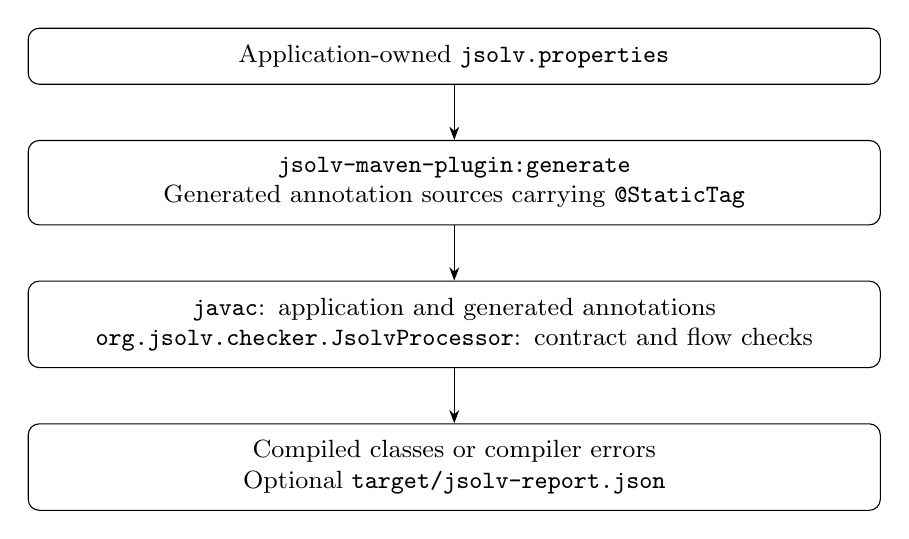
\begin{tikzpicture}[
  box/.style={draw,rounded corners,align=center,text width=10.4cm,
              inner sep=6pt,font=\small},
  node distance=7mm,>={Stealth}]
\node[box] (config) {Application-owned \texttt{jsolv.properties}};
\node[box,below=of config] (generator) {\texttt{jsolv-maven-plugin:generate}\\
  Generated annotation sources carrying \texttt{@StaticTag}};
\node[box,below=of generator] (compiler) {\texttt{javac}: application and generated annotations\\
  \texttt{org.jsolv.checker.JsolvProcessor}: contract and flow checks};
\node[box,below=of compiler] (output) {Compiled classes or compiler errors\\
  Optional \texttt{target/jsolv-report.json}};
\draw[->] (config) -- (generator);
\draw[->] (generator) -- (compiler);
\draw[->] (compiler) -- (output);
\end{tikzpicture}
\caption{JSOLV in the ordinary Maven compilation lifecycle.}
\label{fig:architecture}
\end{figure}

\texttt{JsolvProcessor} extends Java's \texttt{AbstractProcessor}~\cite{processor}.
It obtains syntax paths and resolved compiler elements through the
\texttt{Trees} API~\cite{trees}. A method scanner starts a fresh environment,
seeds parameter contracts, and invokes a flow scanner. The flow state maps
compiler symbols to immutable sets, avoiding confusion between different
variables with the same spelling.

The expression evaluator checks nested calls in initializers, assignments,
receivers, and constructor arguments. It reads labels on both type uses and
declarations. The processor supports all annotation names so application-defined
labels can participate, but returns false from processing so it does not claim
annotations needed by other processors. A service-provider file in the checker
JAR registers \texttt{org.jsolv.checker.JsolvProcessor}.

Generation is deliberately a separate Maven phase, not a first-round side effect
of the checker. This ensures label declarations exist before compilation and
avoids coupling flow analysis to unresolved generated imports.

\subsection{Separate compilation}

CLASS retention preserves annotation metadata for consumers. METHOD and
PARAMETER targets supplement TYPE\_USE metadata. Older javac releases have
limitations exposing class-file type annotations to processors, reflected in
OpenJDK's later fix~\cite{javac-annotations}. Generated labels placed before a
simple return type also annotate the method declaration; the checker consults
that declaration. Regression tests exercise library and consumer compilation
separately on JDK 17. Purely type-use placements should not be assumed to have
the same behaviour on older compilers.

For a multi-module application, generate the vocabulary once in an
application-owned labels JAR. Consumers depend on that JAR and put the checker
on their annotation-processor path. They do not need a local copy of the config
to recognise those labels. Generating identical fully qualified labels in several
modules should be avoided.

\section{Maven setup and reproducible use}
\label{sec:build}

The repository root contains a Maven reactor with annotation, checker,
generator, and demo modules. The \texttt{example-app} directory contains
an independent consumer. The tested
environment uses JDK 17.0.12 and Maven 3.9.11. A JDK is required for compilation
and for tests using \texttt{ToolProvider.getSystemJavaCompiler()}.

From the repository root:
\begin{lstlisting}
mvn -f pom.xml clean install
mvn -f example-app/pom.xml clean compile
\end{lstlisting}
These are local development artifacts, version \texttt{1.0-SNAPSHOT}; this paper
does not assert that they are published on Maven Central. Teams can install them
locally or deploy them to their own artifact repository.

A consuming application needs one dependency:
\begin{lstlisting}[language=XML]
<dependency>
  <groupId>org.jsolv</groupId>
  <artifactId>jsolv-annotations</artifactId>
  <version>1.0-SNAPSHOT</version>
</dependency>
\end{lstlisting}
It also needs the following plugins within \texttt{build/plugins}:
\begin{lstlisting}[language=XML]
<plugin>
  <groupId>org.jsolv</groupId>
  <artifactId>jsolv-maven-plugin</artifactId>
  <version>1.0-SNAPSHOT</version>
  <executions>
    <execution><goals><goal>generate</goal></goals></execution>
  </executions>
</plugin>
<plugin>
  <groupId>org.apache.maven.plugins</groupId>
  <artifactId>maven-compiler-plugin</artifactId>
  <version>3.13.0</version>
  <configuration>
    <release>17</release>
    <proc>full</proc>
    <annotationProcessorPaths>
      <path>
        <groupId>org.jsolv</groupId>
        <artifactId>jsolv-checker</artifactId>
        <version>1.0-SNAPSHOT</version>
      </path>
    </annotationProcessorPaths>
    <compilerArgs>
      <arg>-Ajsolv.report=${project.build.directory}/jsolv-report.json</arg>
    </compilerArgs>
  </configuration>
</plugin>
\end{lstlisting}
The compiler-plugin configuration makes processing explicit~\cite{maven-compiler}.
Omitting the report argument disables reporting without disabling checks.
Generator configuration can override \texttt{configFile} and
\texttt{outputDirectory}; the config path is also selectable through
\texttt{-Djsolv.config=...}. Keep the output dedicated to generated labels.

Use lifecycle commands such as \texttt{mvn compile}. Invoking
\texttt{mvn compiler:compile} directly bypasses the generation phase. IDE users
may need to run \texttt{mvn generate-sources} and reimport the Maven project
before new annotation imports resolve.

\section{Diagnostics and inspectable results}

When a required set is not available, the processor emits a compiler error at
the offending argument. A shortened example is:
\begin{lstlisting}
missing @Authenticated: value lacks required static tags
[org.jsolv.example.tags.Authenticated]
\end{lstlisting}
The full names preserve identity when labels have the same simple spelling.
The prototype reports missing evidence; it does not explain a complete proof
history or reconstruct which earlier branch lost a fact.

The optional JSON report has schema version 2, a processor name, and a
\texttt{checks} array. Each required-argument check records a source URI, line,
column, called method's simple name, one-based argument index, required labels,
known labels, missing labels, and acceptance. For example:
\begin{lstlisting}
{
  "schema": 2,
  "processor": "org.jsolv.checker.JsolvProcessor",
  "checks": [{
    "source": "file:///example/Workflow.java",
    "line": 42, "column": 17,
    "method": "publish", "argumentIndex": 1,
    "required": ["org.jsolv.example.tags.Authenticated"],
    "known": [],
    "missing": ["org.jsolv.example.tags.Authenticated"],
    "accepted": false
  }]
}
\end{lstlisting}
The example illustrates the schema rather than a literal transcript of
\cref{lst:workflow}. Reports include accepted and rejected required-argument
checks and are written at the final processing round. They do not enumerate
all expressions or all diagnostics. Invalid Java can prevent processing from
reaching this stage. An up-to-date Maven compile may skip javac and leave the
previous report; \texttt{clean compile} produces a fresh compilation.

\section{Trust boundaries and limits of enforcement}
\label{sec:limits}

Label generation does not generate the domain operation. A truthful
\texttt{@Validated} method must actually establish the application's definition
of validation. An \texttt{Authenticated} label is not intrinsically tied to a
principal, resource, policy, or time. Such context must be represented in the
application contract; parameterised labels are not implemented.

The prototype checks calls against contracts but does not verify return
statements against promised result labels, infer method summaries, or check
override compatibility. A false annotation can therefore cause acceptance of
an invalid domain workflow. Auditing introducing and preserving methods is an
essential part of adoption.

\subsection{Bindings are not a heap analysis}

Copying a binding copies its tracked facts. Reassigning one binding leaves
another binding's tracked facts intact. This models value provenance for local
variables, not mutable object state shared by references. Consider:
\begin{lstlisting}[language=Java]
Document saved = persist(document);
Document alias = saved;
alias.setContents("different content");
publishSaved(saved);
\end{lstlisting}
If persistence depends on the current contents, the old fact may now be false.
The checker does not automatically revoke it after the mutating call. Immutable
data and reviewed transformation contracts fit the prototype much better than
arbitrary mutable protocols. Immutability alone also does not make an incorrect
preservation annotation true.

\subsection{Control flow and unsupported constructs}

\texttt{if} and conditional-expression joins use intersections. Loops,
try/catch/finally, and switch statements conservatively forget facts for assigned
variables and do not establish new facts after the construct; switch cases and
exception branches are inspected separately. The processor does not build a
complete control-flow graph or compute loop fixed points. Early returns,
break/continue, exceptions, and reachability do not prune joins. Safe programs
may therefore be rejected.

Fields and array elements supply no known label facts. Generic element flow,
receiver contracts, method references, streams, and asynchronous callbacks are
not modelled. Lambda bodies start separate state with parameter contracts and
unknown captured facts. Switch expressions supply no result facts and clear
tracked state. An annotated array passed as a single varargs argument is not
modelled like a sequence of individually checked values. Initializers outside
method bodies are outside the current scans.

Conservative treatment of some constructs does not establish global soundness.
The unmodelled effects and mutable-alias example already preclude such a claim.
The actual guarantee is a useful collection of supported contract and flow
checks, not a security proof for arbitrary Java.

\section{Relationship to the broader proposal and other techniques}

\Cref{tab:scope} distinguishes what \jsolv{} implements from the wider static
property proposal. This separation avoids interpreting a convenient annotation
syntax as a claim that difficult analysis problems have been solved.

\begin{longtable}{@{}>{\raggedright\arraybackslash}p{0.36\linewidth}
                      >{\raggedright\arraybackslash}p{0.58\linewidth}@{}}
\caption{Scope of the present implementation.}\label{tab:scope}\\
\toprule
Concept & JSOLV status \\
\midrule
\endfirsthead
\toprule Concept & JSOLV status \\ \midrule
\endhead
User-defined positive atomic labels & Implemented through configuration and generated annotations. \\
Value-flow requirements and result contracts & Implemented for the documented local fragment; result contracts are trusted. \\
Independent label composition & Implemented by sets and explicit single-input preservation. \\
Negative facts and requirements & Not implemented; absence means unknown. \\
Validator Boolean branch refinement & Not implemented; call result contracts establish facts on returned values. \\
Alias-aware or effect-based revocation & Not implemented. \\
Full CFG and loop fixed points & Not implemented. \\
Parameterised labels and implications & Possible extensions, not configuration features today. \\
Proof-producing or verified validators & Possible extensions; current boundaries are trusted. \\
\bottomrule
\end{longtable}

\jsolv{} overlaps with pluggable type qualifiers, typestate, and taint analysis.
The Checker Framework demonstrates a substantially richer approach to pluggable
Java checking~\cite{checker-framework}; \jsolv{} does not claim equivalent
coverage or qualifier polymorphism. Its set-based facts are independent rather
than one enumerated protocol state, and its core vocabulary is domain-neutral.
It can resemble an opaque refinement layer, but it has no general predicates,
solver, or proof language.

Compared with wrappers, labels preserve the ordinary API and avoid introducing
combination-specific classes. Wrappers can provide stronger nominal separation
and carefully controlled construction, so the mechanisms are complementary.
The architectural distinction advocated by the semantic-categories paper is
realised here without changing Java's parser or runtime representation.

\section{Regression evidence and evaluation boundaries}

The current regression suite contains 24 tests: three generator tests,
four original persistence-checker tests, and seventeen configurable-label tests.
The renamed JSOLV build passes these tests in the stated JDK/Maven environment.
The independent application exercises actual Maven goal binding, service-based
processor discovery, generated imports, and JSON reporting.

The tests cover configuration validation, owned-file cleanup, unchanged output,
multiple simultaneous requirements, explicit and selected-argument preservation,
loss after unannotated transformation, parameter forwarding, branch intersection,
casts, scope identity, nested calls, constructor arguments, expanded varargs,
selected control-flow cases, reports, and separately compiled libraries. One
test adds a new configuration label, generates its annotation, compiles a valid
use, and rejects a missing-label use without changing the checker. Another
distinguishes equally spelled labels from different packages.

These are regression observations, not an empirical demonstration of defect
reduction, acceptable false-positive rates, or scalability. No developer study,
large-codebase benchmark, or compilation-overhead measurement is reported.
The next evaluation should measure annotation burden, unsupported-pattern
frequency, compilation cost, and whether diagnostics help developers repair
real workflows without adding incorrect trust contracts.

\section{Adoption and future development}

A useful adoption order is to identify a few meaningful sinks, annotate their
requirements, and review the methods that genuinely establish those facts.
Then introduce preservation only where every existing fact remains true for
the result. Prefer immutable values, narrow contracts, and application-owned
label packages. In a shared library, publish the generated vocabulary once.

Future analysis work should prioritise a complete control-flow representation,
effect-aware invalidation, override checks, and verified result contracts before
claiming stronger guarantees. Selective preservation would help transformations
that retain some facts while invalidating others. Contextual or parameterised
labels could express authorisation for a particular resource, but require a
precise identity model. Label implications should likewise have explicit,
bounded semantics rather than unrestricted rules hidden in configuration.

The two-key vocabulary and marker protocol need not change as analysis improves.
Keeping application naming separate from compiler logic lets the tool develop
without transferring checker-maintenance responsibilities to application teams.

\section{Conclusion}

\jsolv{} makes a useful subset of static property tagging available in ordinary
Java. Application teams name their facts in a small configuration file, generated
annotations expose those facts in signatures, and a generic checker enforces
supported value-flow requirements during compilation. Explicit preservation
allows independent workflow stages to compose without a family of nominal
types or a registry embedded in checker code.

The design's effectiveness comes from a clear division of responsibilities:
applications own vocabulary and truthful contracts; generation supplies ordinary
Java declarations; analysis transports sets of known facts; diagnostics expose
missing evidence. Its limits are equally explicit. The implemented tool is a
practical workflow checker with trusted boundaries, and a foundation for stronger
analysis, rather than a completed solution to arbitrary object-state verification.

\begin{thebibliography}{9}
\raggedright
\bibitem{property-tags}
Sambuddha Majumder and Jayanta Majumder.
\emph{User-Defined Static Property Tags for Mainstream Programming Languages:
A Lightweight Flow-Sensitive Verification Layer}.
Companion manuscript, \texttt{static\_property\_tags.tex}.

\bibitem{semantic-categories}
Jayanta Majumder and Sambuddha Majumder.
\emph{Explicit Semantic Categories for More Legible Mainstream Programming Languages}.
Companion manuscript, \texttt{semantic\_roles\_beyond\_class.tex}.

\bibitem{processor}
Oracle. \emph{Java SE 17 API: AbstractProcessor}.
\url{https://docs.oracle.com/en/java/javase/17/docs/api/java.compiler/javax/annotation/processing/AbstractProcessor.html}

\bibitem{trees}
Oracle. \emph{Java SE 17 API: Trees}.
\url{https://docs.oracle.com/en/java/javase/17/docs/api/jdk.compiler/com/sun/source/util/Trees.html}

\bibitem{maven-lifecycle}
Apache Maven. \emph{Introduction to the Build Lifecycle}.
\url{https://maven.apache.org/guides/introduction/introduction-to-the-lifecycle.html}

\bibitem{maven-compiler}
Apache Maven. \emph{Maven Compiler Plugin 3.13.0: compiler:compile}.
\url{https://maven.apache.org/plugins-archives/maven-compiler-plugin-3.13.0/compile-mojo.html}

\bibitem{javac-annotations}
OpenJDK. \emph{Type annotations are not visible to javac plugins across
compilation boundaries}, JDK update discussion, March 2025.
\url{https://mail.openjdk.org/pipermail/jdk-updates-dev/2025-March/041891.html}

\bibitem{checker-framework}
The Checker Framework developers. \emph{The Checker Framework}.
\url{https://checkerframework.org/}
\end{thebibliography}

\end{document}
